\clearpage
\section{Introduction to the Robot Maze}

The coursework exercises for this year's CS118 module are based on a simulated ``Robot Maze'' environment.  A small robot has been designed to be able to navigate its way through mazes to find a target at some given location.  This task resembles those used in the classic learning 
experiments of the 1960s which included laboratory
mice (and cheese, mild electric shocks, mice of the opposite sex, etc).
The objective of the robot (or mouse as it was then) or, more generally, the \emph{agent} is to 
find the given target as rapidly and efficiently as
possible, learning the maze over several runs and so on.  

Building a real robot and a real maze requires a combination of efficient 
sensors and mechanics, sophisticated steering and speed control, clever 
maze exploration and navigation procedures and, no doubt, a good deal of
glue.  For the purpose of these exercises we focus
entirely on designing the maze exploration and navigation algorithms.
We make no attempt to model the physics of a moving wheeled (or legged!)
robot and concentrate solely on the part of the 
problem which can best be solved with software. 

\subsection{The Robot Maze environment}

The simulated Robot Maze environment has the following characteristics:

\begin{itemize}

\item The robot moves through a simple square-block maze of the type
  illustrated in \Cref{maze}.  The floor space of the maze is divided into squares of uniform size. Each square is either occupied by a wall or is empty.

\item The robot occupies exactly one non-wall square and moves in
  discrete steps, one square at a time, north, south, east, or west.
  The robot cannot move diagonally.  If the robot attempts to move
  outside the boundary of the maze or into squares occupied by walls it
  suffers a harmless collision (indicated by flashing red in the
  simulation) and stays in the same square.

\item The direction the robot moves in is determined by the direction it is facing (its heading, indicated by an arrow in the simulation).  The robot can change the direction it is facing by rotating on the spot. Each of these rotations are directed by the robot's control procedure -- a method called \javaIn{start} -- which is run at the start of a simulation. 

\item A simulation \emph{usually} starts with the robot at the top left-hand square of the maze and ends when either the robot reaches the target or the user loses patience and stops the robot (by pressing {\bf Reset} in the user interface). The target square is usually the bottom right-hand corner of the maze, but this along with the robot start position can be modified by the user. 

\end{itemize}

\begin{figure}
\centering
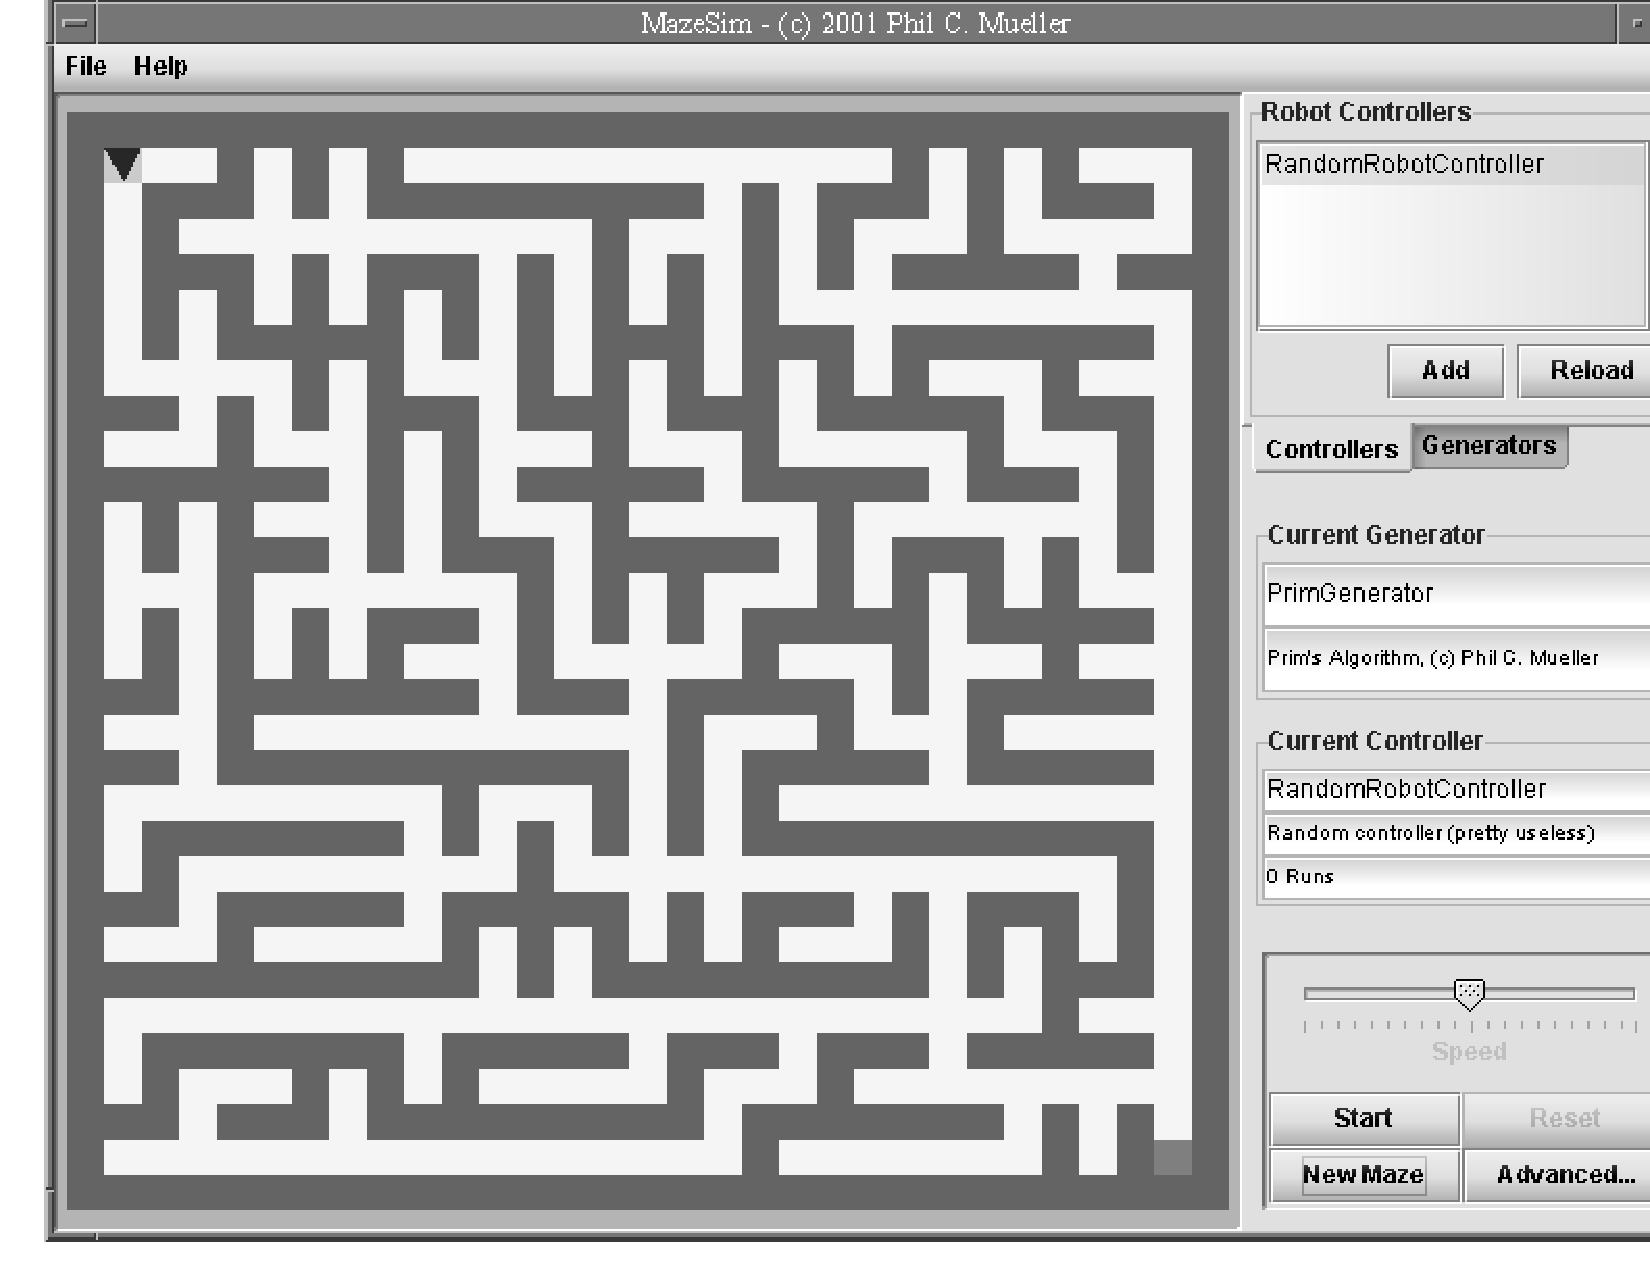
\includegraphics[width=10cm]{maze.pdf}
\caption{The Robot-maze environment\label{maze}}
\end{figure}

During its execution the robot's control program (which you are required to
write) has access to the following information:

\begin{itemize}

\item The direction the robot is currently facing;

\item The status of the squares ahead, behind, left and to the right of the robot. Squares are either walls, empty, or squares the robot has been at before (which are otherwise empty squares). The boundaries of the maze are treated as walls;

\item The {\it x} and {\it y} co-ordinates of the square the robot is currently occupying, and those of the target square;

\item How many attempts the robot has made at traversing the given maze.
\end{itemize}

\subsection{Programming robot control programs}

The simulated robot maze environment is written in Java. The programs which you are required to write for this module are also Java-based which means that you will be writing code which directly hooks into this robot maze environment. 

To allow this hook-up, there needs to be a common interface between the robot maze Java code and your own Java code. This interface is documented in the following sections. However, since you are only required to write control software for the maze environment and while every part of the maze software is accessible for you to use, the implementation of the maze environment itself is hidden from you. This is an example of abstraction. Everything you need to know to use the maze environment is documented in this guide.

The information listed below is important and you should make sure that you understand what it all means. If you are not clear on anything then you might like to talk about it with your peers first and then ask for clarification from the teaching team. Understanding \emph{program interfaces} like this is very important in software development, particularly if you are to use it to write your own program code.

\subsubsection{Specifying headings in the maze}

Four pre-defined constants are defined in the code for the robot maze program to specify directions in the maze. These are

\javaIn{IRobot.NORTH}, \javaIn{IRobot.EAST}, \javaIn{IRobot.SOUTH}, \javaIn{IRobot.WEST}

where the maze follows the usual mapping convention of having \javaIn{IRobot.NORTH} upwards and \javaIn{IRobot.EAST} to the right etc.

As the values are defined as part of a Java interface named \javaIn{IRobot}, the constants are prefixed with the name of the interface as shown above when they are used in the actual program code that you write. This might seem a bit quirky but you will 
soon get used to it. 

These elements of the interface are concretely represented as Java values of type \javaIn{int}. The values represented by these directional constants are chosen so that the following equalities hold:

\begin{center}
\begin{tabular}{rcl}
\javaIn{IRobot.NORTH+1} & \javaIn{==} & \javaIn{IRobot.EAST}	\\ 
\javaIn{IRobot.EAST+1} & \javaIn{==} & \javaIn{IRobot.SOUTH}	\\ 
\javaIn{IRobot.SOUTH+1} & \javaIn{==} & \javaIn{IRobot.WEST}	\\ 
\end{tabular}  
\end{center}

\taskLine 

\task{Note that \javaIn{IRobot.WEST+1 != IRobot.NORTH}. Could you find a way to represent the directions in Java so that this would be the case?}

\taskLine 

\subsubsection{Specifying directions relative to the robot heading}

Four pre-defined constants are defined in the code for the robot maze program to specify directions relative to the robot's current heading. These are:

\javaIn{IRobot.LEFT}, \javaIn{IRobot.RIGHT}, \javaIn{IRobot.AHEAD}, \javaIn{IRobot.BEHIND}

As with headings these are also of the type \javaIn{int}. The values represented by these directional constants are chosen so that the following equalities hold::

\begin{center}
	\begin{tabular}{rcl}
		\javaIn{IRobot.AHEAD+1} & \javaIn{==} & \javaIn{IRobot.RIGHT}	\\ 
		\javaIn{IRobot.RIGHT+1} & \javaIn{==} & \javaIn{IRobot.BEHIND}	\\ 
		\javaIn{IRobot.BEHIND+1} & \javaIn{==} & \javaIn{IRobot.LEFT}	\\ 
	\end{tabular}  
\end{center}

A fifth constant \javaIn{IRobot.CENTRE} is also defined, which can be useful as a ``do nothing'' value when communicating values between parts of complex control programs.

Do not be put off by the fact that these values have an \javaIn{int} type. As far as the control programmer (this is you) is concerned, all references to headings and directions are done using the constant \emph{name} (i.e. \javaIn{IRobot.RIGHT}, 
\javaIn{IRobot.NORTH}, etc.) and not the constant \emph{value} used to represent it. This is our first encounter with \emph{program abstraction}. 

\subsubsection{Sensing the squares around the robot}
\label{lookmethod}

The method \javaIn{robot.look(direction)} takes a value
specifying a direction relative to the robot (e.g. \javaIn{IRobot.AHEAD} or \javaIn{IRobot.LEFT}, etc.) and returns a value which indicates the state of the corresponding square neighbouring the robot. The possible states are:

\begin{tabular}{r|p{0.6\textwidth}} 
	\javaIn{IRobot.PASSAGE} &  An empty square that has not yet been visited on the current traversal of the maze. \\ \hline 
	\javaIn{IRobot.WALL} & An empty square that
	has already been visited during the current traversal of the maze. \\ \hline  
	\javaIn{IRobot.BEENBEFORE} & A wall or the edge of the maze \\
\end{tabular} 

\begin{figure}
\begin{subfigure}[t]{0.5\textwidth}
	\centering
	\includegraphics[width=0.5\textwidth]{mousemove_new}
\end{subfigure} 
~
\begin{subfigure}[t]{0.5\textwidth}
	\centering
	\begin{tabular}{l l} 
		\textbf{Function call} & \textbf{Result} \\ \hline
		\javaIn{robot.look(IRobot.AHEAD)}  & \javaIn{IRobot.WALL} \\
		\javaIn{robot.look(IRobot.BEHIND)} & \javaIn{IRobot.BEENBEFORE} \\
		\javaIn{robot.look(IRobot.LEFT)}   & \javaIn{IRobot.WALL} \\
		\javaIn{robot.look(IRobot.RIGHT)}  & \javaIn{IRobot.PASSAGE} 
	\end{tabular}
\end{subfigure}

\caption{Example of sensing robot surroundings\label{sensing}}
\end{figure}

\Cref{sensing} shows a typical situation that might arise during a
traversal of the maze. The robot is located in the square with an arrow, facing in the direction of the arrow, with squares visited previously during the same run shaded in grey. The walls are in black. In this situation \javaIn{robot.look} would return the results shown in the table.

If the robot chooses to turn right and then move forward one square, then a call to the method \javaIn{robot.look(IRobot.AHEAD)} would return \javaIn{IRobot.PASSAGE}.

\subsubsection{Sensing and setting the robot's heading}

The method \javaIn{robot.getHeading()} returns the robot's current heading in the maze. That is either \javaIn{IRobot.NORTH}, \javaIn{IRobot.SOUTH}, \javaIn{IRobot.EAST}, or 
\javaIn{IRobot.WEST}. In the example in \Cref{sensing} a call to the method \javaIn{robot.getHeading()} would return the value \javaIn{IRobot.EAST}. There is a ``sister'' method called \javaIn{robot.setHeading(x)}, which can be used to set the robot's heading (where the parameter \javaIn{x} is 
one of \javaIn{IRobot.NORTH}, \javaIn{IRobot.SOUTH}, \javaIn{IRobot.EAST} or \javaIn{IRobot.WEST}).

\subsubsection{Sensing the location of the robot and target}

The method \javaIn{robot.getLocation()} returns an object of type \javaIn{Point} which has two public variable members. You can get the $x$ and $y$ coordinates of the robot in the maze from
the \javaIn{Point} class by accessing the \javaIn{x} and \javaIn{y} members of the object:
\begin{minted}{java}
Point p = robot.getLocation();
System.out.println("The robot is at " + p.x + " and " + p.y);
\end{minted}
Did you know that you could also write the following instead:
\begin{minted}{java}
System.out.println("The robot is at " + 
    robot.getLocation().x + " and " + 
    robot.getLocation().y);
\end{minted}
The top left square in the maze is represented by the coordinates $(1,1)$. Similarly, the method \javaIn{robot.getTargetLocation()} can be used to return the $x$ and $y$ coordinates of the robot's target.

\subsubsection{Turning the robot}

The method \javaIn{robot.face(direction)} makes the robot turn in the specified \javaIn{direction} (one of \javaIn{IRobot.AHEAD}, \javaIn{IRobot.BEHIND}, \javaIn{IRobot.LEFT}, or \javaIn{IRobot.RIGHT}) relative to its current heading.  
The turn is performed immediately and will be reflected in the results of subsequent calls to \javaIn{robot.getHeading()}.

\subsubsection{Moving the robot}

Your code should point the robot in a suitable direction. Afterwards, you should instruct the robot to advance into the specified direction. The \javaIn{robot.advance()} method will cause the robot to move by one square into the direction that it is facing. For example, the following code would cause the robot to turn right and advance into the resulting direction by one square:

\begin{minted}{java}
robot.face(IRobot.RIGHT);
robot.advance();
\end{minted}

\subsubsection{Detecting the start of a traversal and a change of maze}

The method \javaIn{robot.getRuns()} returns a value of type \javaIn{int} which corresponds to the the number of previous traversals which the robot has made of a given maze.  After you have guided a robot through a maze, you will notice that the user interface of the robot maze environment displays 
\texttt{1 Run} on the right. This is the result of the \javaIn{robot.getRuns()} method. You will find that this method is useful in the second coursework.




